\chapter{Multi-modeling in MATSim: PSim}
\label{ch:psim}
% ##################################################################################################################

\hfill \textbf{Author:} Pieter Fourie

\begin{center} 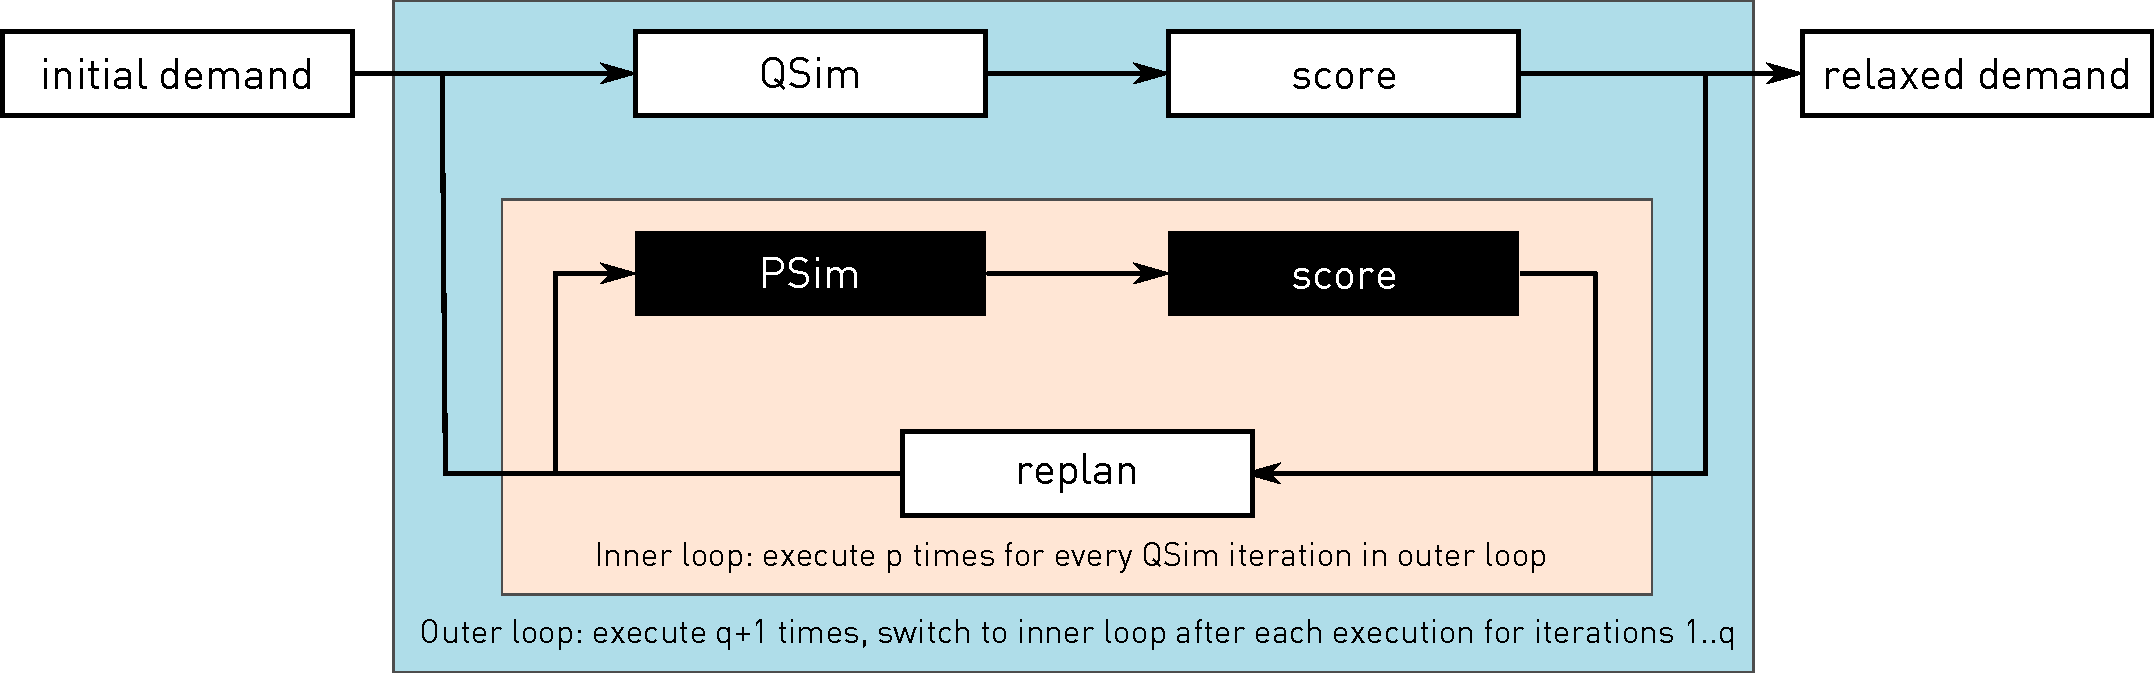
\includegraphics[width=0.5\textwidth, angle=0]{extending/figures/PSim/psim.pdf} \end{center}

\createStandardInformation{todo}{todo}{todo}{\citet[][]{FourieEtAl_TRR_2013}}

% ##################################################################################################################
\section{Introduction}
The greatest current performance limitation to MATSim is the network loading simulation, i.e., the mobsim, for example QSim or JDEQSim. This chapter is focused on QSim. As shown earlier, QSim is repeatedly executed in the MATSim cycle for the entire agent population (Section~\ref{sec:inbrief}).

With the multi-modeling approach \citep[][]{FourieEtAl_TRR_2013}, shown in Figure~\ref{fig:PSim}, a MATSim run periodically replaces QSim for a number of iterations with a simplified meta-model or pseudo-simulation (PSim) that runs approximately two orders of magnitude faster. In risk analysis these models are called "surrogate models" \citep[][]{Sudret_APSSRA_2012}. PSim uses travel time information from the preceding QSim iteration to estimate how well an agent day plan might perform, and allow multiple iterations of mutation and evaluation between QSim iterations to more rapidly explore the agents' solution space, thereby producing better performing plans in a shorter time.

% ------------
\createfigure%
{Operation of a MATSim run implementing pseudo-simulation}%
{Operation of a MATSim run implementing pseudo-simulation}%
{\label{fig:PSim}}%
{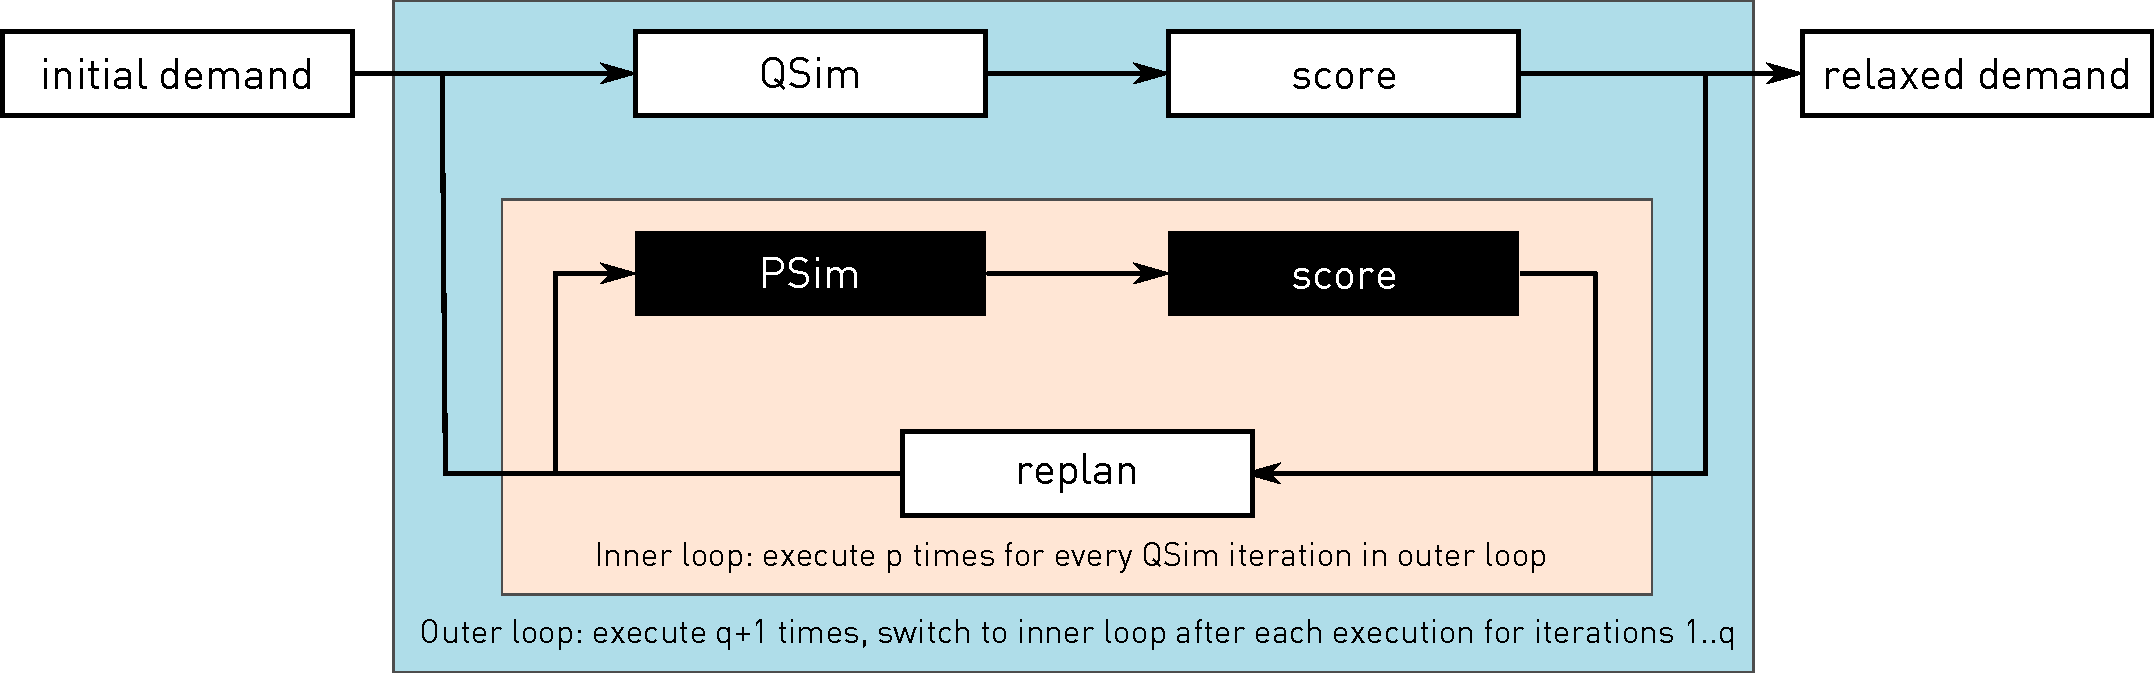
\includegraphics[width=0.7\textwidth, angle=0]{extending/figures/PSim/psim.pdf}}%
{}
% ------------

% ##################################################################################################################
\section{Basic Idea}
PSim exploits the classes that record various aspects of network performance during queue simulations and uses them as an approximate meta-model of QSim. It fires the exact same sequence of events for car and public transport passengers as is produced during a QSim mobility simulation, with the exception that event timings are approximate values that can be expected for the time of day in which they occur.

For private vehicle traffic, it calls the \lstinline|getLinkTravelTime(Link link, double time, Person person, Vehicle vehicle)| method of classes implementing the \lstinline|TravelTime| interface to fire \lstinline|LinkEnterEvents| and \lstinline|LinkLeaveEvents| at appropriate times for all the links in a car route. For public transportation, the events sequence generated for a passenger traveling on a particular service rely on a meta-model of stop-to-stop travel times (\lstinline|interface StopStopTime|) and waiting times at stops (\lstinline|interface WaitTime|), both of which are concepts developed by Sergio Ord\`o\~nez at the Future Cities Laboratory (package \lstinline|playground.singapore.transitRouterEventsBased|).

PSim plans are scored using the same scoring function as that of QSim iterations, and is compatible with most replanning modules in MATSim. Following a series of PSim iterations, a plan is selected for each agent in the usual fashion and a QSim iteration is run to start a new cycle. The various classes used in PSim are updated with the latest network performance information, and the process repeats.

% ##################################################################################################################
\section{Performance}
Initial tests on the Zürich scenario (described in Section~\ref{sec:zhscenario}) have shown a dramatic decrease in computation times compared to the default QSim-only approach, with performance improving linearly with an increasing number of computational cores.
Figure \ref{fig:PSimPerformance} compares the PSim-approach in two configurations against the existing approach, for a 10\,\% sample of private vehicle traffic in Zürich. All simulations were run until they reached a target score, i.e.,\,the score reached after running the standard approach for 100\,iterations. The first PSim-implementing configuration uses the same rate of plan mutation as the QSim-only approach, where 30\,\% of agents are selected for plan mutation (replanning) after each iteration, whether it is a QSim or PSim iteration. The new approach requires fewer QSim iterations to reach a target score, but requires more time for replanning. Replanning is fully multi-threaded, with no synchronization between cores required, so it’s performance increases linearly with increasing number of cores, so times improve more dramatically for the new approach than the standard approach.
In the second configuration, the mutation rate is reduced and the number of PSim iterations between QSim iterations increased to 24 for each QSim iteration. The system now tests many more combinations of different mutation operations (4 in this case: activity timing, mode choice, secondary activity location choice, and re-routing), to reach the target state in a much quicker time, even though it produces a smaller expected number of mutated plans per agent between QSim iterations (3 for configuration 1, 2.5\,plans for configuration 2).

This last point raises an interesting issue; namely that the distribution of the number of mutation operations can be dramatically spread out with the PSim approach, because increasing the number of iterations is relatively cheap. This should make the approach favorable with especially random mutation-producing replanning strategies, where a large number of mutations are needed to produce a relaxed simulation state.

For a detailed discussion of the meta-modeling approach and the results of applying this method to the Zürich scenario, refer to \citet[][]{FourieEtAl_TRR_2013}.

% ------------
\createfigure%
{PSim computation time}%
{Computation time contributions vs. number of computational cores for QSim-only (0.3 replanning rate), 9\,PSim iterations per QSim iteration at 0.3\,replanning rate, and 24\,PSim iterations per Qsim iteration at 0.1\,replanning rate}%
{\label{fig:PSimPerformance}}%
{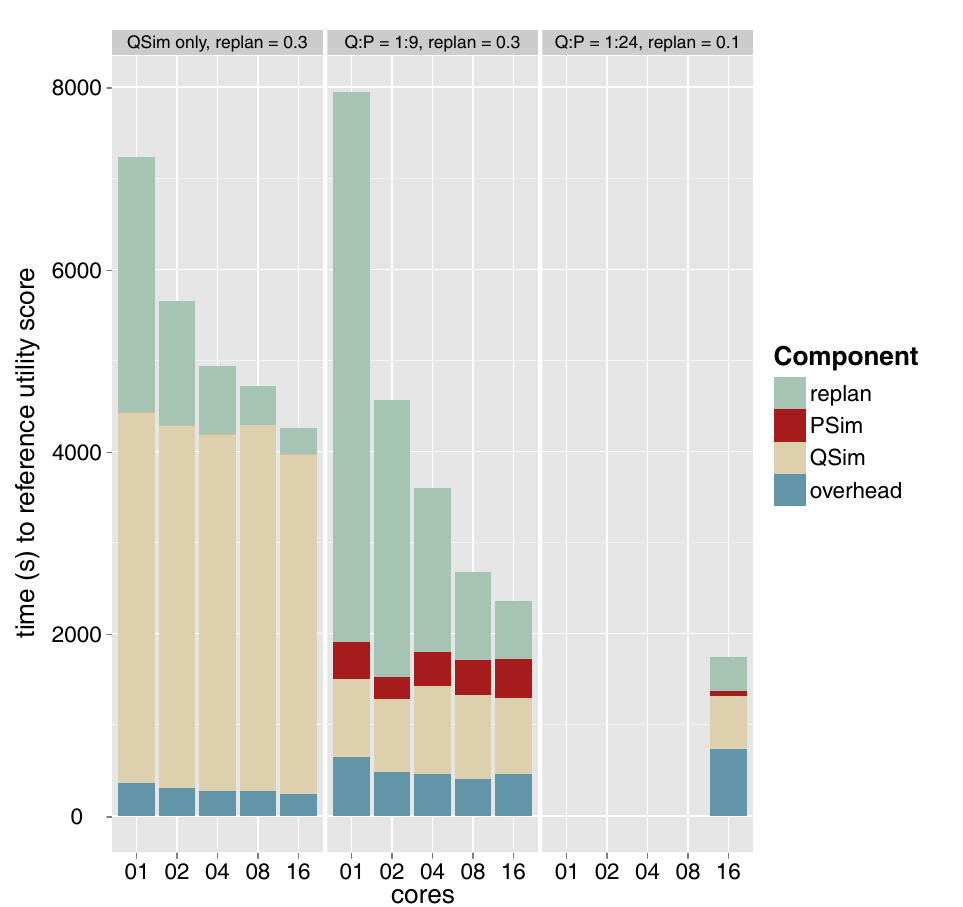
\includegraphics[width=0.7\textwidth, angle=0]{extending/figures/PSim/times}}%
{}
% ------------

% ============================================================================================
\subsection{Distributed Computing}
Because PSim executes plans independently from each other, requiring no coordination of computational processes, it is possible to distribute it across multiple nodes with no need of shared memory, as illustrated in Figure~\ref{fig:distributedPSim}. To this end, we (Fourie and Ord\`o\~nez, Future Cities Laboratory) are implementing a simple messaging protocol to transmit network performance objects to PSim slave nodes from a master node running QSim only. Slave nodes perform replanning operations and evaluate plans in a pre-determined number of PSim iterations per cycle. At the start of each QSim iteration, a single plan for each agent is transmitted back to the master from all the slaves, and updated \lstinline|TravelTimes, StopStopTimes and WaitTimes| are rendered during the full mobility simulation, to be transmitted back to the slaves in the next cycle.

The approach yielded promising results, with a reduction in the number of QSim iterations as in the previous work, as well as the potential for running large-scale simulations on much cheaper hardware than the current approach that demands expensive shared memory servers. Most importantly, all replanning takes place in parallel with the QSim running on the master, so the time spent waiting for replanning operations can be reduced to nil. This performance increase is especially useful for large scenarios implementing public transportation, where the time spent replanning can be up to twice that of the queue simulation.

% ------------
\createfigure%
{Master-slave configuration for running PSim}%
{Master-slave configuration for running PSim in distributed mode, across many slave computer nodes in a local area network or in a cloud computational framework. The master runs selected plans in a full queue simulation, and transmits updated travel time information to slave nodes after every iteration. In turn, slaves produce and evaluate new plans in repeated PSim/replanning cycles, sending the master a single plan for each agent at the start of a QSim iteration}%
{\label{fig:distributedPSim}}%
{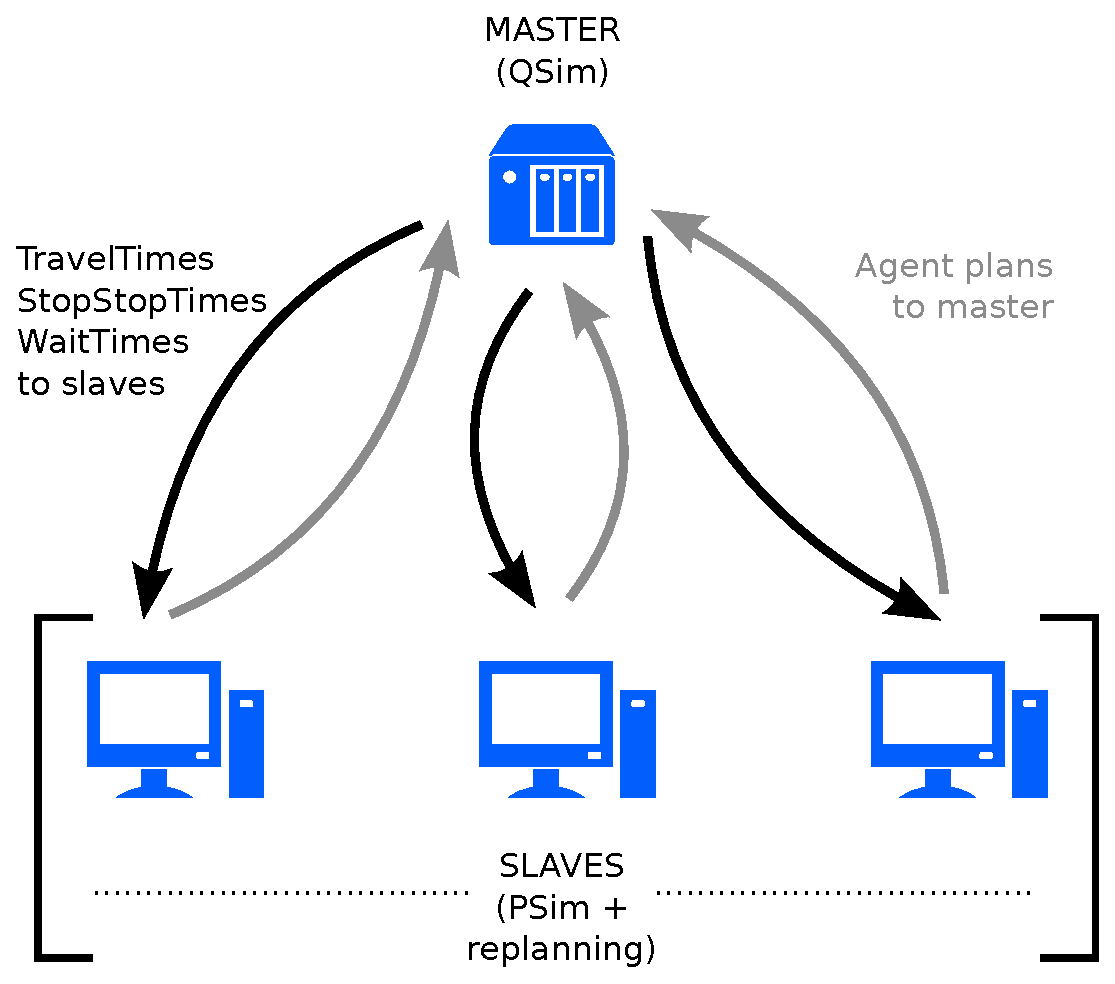
\includegraphics[width=0.7\textwidth, angle=0]{extending/figures/PSim/distributed}}%
{}
% ------------

% ##################################################################################################################